\documentclass[../dissertation.tex]{subfiles}

\begin{document}

\chapter{Critical Evaluation}

\label{chap:evaluation}

Here, a range of techniques are used to evaluate the benefits of the newly proposed Neural-Q path tracer compared to the Expected Sarsa path tracer presented in Chapter \ref{chap:td_deep_sampling}. However, it is also made clear that Neural-Q's viability in current industry is limited due to the time taken to evaluate a forward pass through an ANN.

\section{Experimental Setup}

A path tracing renderer was built from scratch which supported Algorithms \ref{alg:forward_path_tracing}, \ref{alg:expected_sarsa_pathtracer}, \ref{alg:neural_q_pathtracer} and was used to produce all rendered results seen in this thesis. The rendering engine used only OpenGL Mathematics library \cite{glm} for various operations that are common in the rendering pipeline, SDL2 \cite{sdl2} for displaying rendered images, and the Dynet neural network library \cite{dynet} for the Neural-Q path tracer implementation. Algorithms \ref{alg:forward_path_tracing}, \ref{alg:expected_sarsa_pathtracer}, \ref{alg:neural_q_pathtracer} were all accelerated on an Nvidia GPU by using the CUDA Toolkit \cite{cuda} to receive experimental results in an acceptable time. The reasoning for choosing Dynet over more commonly used neural networks libraries such as Tensorflow \cite{tensorflow2015-whitepaper}, was due to its ability to be easily compiled with the CUDA \verb|nvcc| compiler and it had a well documented C++ API. This was a requirement for the Neural-Q path tracer as tracing light paths, ANN inference, and ANN training are all performed on a Nvidia GPU via C++ API calls. All results were produced using a machine with an Intel i5-8600K CPU, Nvidia 1070Ti GPU and 16GB of RAM installed.\\

I developed four different scenes using Maya \cite{maya} and created a custom object importer to import the scenes into my path tracer renderer. A reference image of all four scenes is given in Figure \ref{fig:mape_results_grid}, which have been rendered with 4096 sampled light rays per pixel using the default forward path tracing Algorithm \ref{alg:default_path_tracer}. They are known as reference images as they have minimal visible noise, meaning the Monte Carlo approximations for each pixel's colour value has approximately converged. Each rendered image from any of the techniques has been rendered at a resolution of 720X720. Due to path tracing accurately modelling physical light transport (see section \ref{sec:mc_pathtracing}), these images are the ideal case for which all other path tracing algorithms should aim to produce as closely as possible with as few samples as possible. 

\section{Assessing the reduction in image Noise for Monte Carlo Path Tracing}

Importance sampling techniques are used in Monte Carlo path tracing to ultimately reduce image noise using the same number of sampled light paths per pixel. Therefore, the most important point to assess is if the Neural-Q path tracer is able to reduce image noise to the same extent as the Expected Sarsa path tracer when using the same SPP. 

\subsection{Quantifying the Reduction in Image Noise}

To quantify the amount noise within images rendered by a default forward path tracer, the Expected Sarsa path tracer, and the Neural-Q path tracer, I will use the Mean Absolute Percentage Error (MAPE) given in Equation \ref{eq:mape} \cite{muller2018neural}.

\begin{equation}
\label{eq:mape}
M = \frac{1}{N} \sum_{i=0}^{N-1} \left| \frac{A_i - F_i}{A_i} \right|
\end{equation}

\noindent
Where:
\begin{conditions}
N & The total number of pixels in the image\\
A_i & The $i$th pixel value in the reference image\\
F_i & The $i$th pixel value in the image whose noise is being quantified\\
\end{conditions}

The MAPE value can then be used to quantify the average difference between pixel values from the reference image to each image rendered by the three path tracing algorithms with the same number of SPP. Therefore, a lower MAPE score is more desirable for a rendered image, as it means the image has a lower amount of noise. The MAPE score for images rendered by the three different path tracing algorithms for four different scenes  is shown in \ref{fig:mape_results_grid}. Each one of the four different scenes have been designed to exhibit different properties which affect light transport simulation, which can be summarised as:\\

\begin{itemize}
\item \textbf{Shelter} - A large scene which includes three different area lights, each with their own blockers. This makes it difficult to learn the contribution of radiance from each of the three sources to a given point in the scene. The scene is a sealed room, meaning all light paths will intersect with an area light as the number of reflections tend to infinity.

\item \textbf{Cornell Box} - A ubiquitous scene to test the accuracy of a rendering techniques approximation of global illumination. The scene is small and includes two light blockers. The wall in the directions of the camera is missing, meaning there is a void which causes light paths to potentially never intersect with an area light.

\item \textbf{Complex Pillars} - A scene which poses a true challenge to estimating the incident radiance on a point, due to the number of light blockers. The scene is sealed and the left, right, bottom, and top walls are all made to absorb most of the light incident on them. Meaning, light paths must navigate through the pillars to illuminate the back walls of the scene and the pillars themselves.

\item \textbf{Door Room} - The door room is a sealed scene which is almost entirely lit by indirect illumination. Light paths must reach the light before their contribution to the final image becomes negligible. 
\end{itemize}

From the MAPE score calculated for each rendered image of the four scenes using the three different path tracers, it is clear that the default forward path tracer in Algorithm \ref{alg:default_path_tracer} is inferior to the path tracers which leverage the power of importance sampling in light path construction. Meaning, the Expected Sarsa and Neural-Q algorithms have both learnt an approximation of the incident radiance distribution function $L_i(x, \omega)$ for each scene, such that it is closer to normalizing the numerator in the Monte Carlo integration computed by path tracing (Equation \ref{eq:rendering_eq_monte_carlo}). This causes a reduction in variance for the estimate of a pixel's colour value by the path tracing algorithms, leading to a lower amount of image noise within the renders displayed in \ref{fig:mape_results_grid}.\\

The MAPE scores for the Neural-Q path tracer are significantly lower for the Shelter and Complex pillars scenes compared to the Expected Sarsa algorithms, and a tie is essentially reached for the Door Room scene. Whereas, the Expected Sarsa clearly beats the Neural-Q path tracer for MAPE score on the Cornell Box. Based on the MAPE calculation, the Neural-Q path tracer outperforms the Expected Sarsa path tracer for larger scenes with more complex geometry and a greater number of area light sources for reducing image noise using less memory. The memory usage of the methods is discussed in detail in \ref{sec:mem_to_comp}, where the actual amount of memory used to produce each of the rendered scene images from both the Neural-Q and Expected Sarsa method are given in \ref{tab:memory_usage}. On the other hand, for smaller scenes with less complex geometry and a lower number of area light sources, the Expected Sarsa algorithm performs comparably well if not better. My hypothesis behind why this is, is that the reduction in noise is largely due to the Neural-Q's ability to generalize the approximation of the incident radiance distribution at any position in the scene, and that this is more important for larger complex scenes. This hypothesis is discussed in more detail in sections \ref{sec:close_inspec_pixels} and \ref{sec:convergence_learning_incident}.

\begin{figure}[hbtp]
\begin{center}
\includegraphics[width=0.9\textwidth]{images/noise_reduction.png}    
\end{center}
\caption{A comparison of the default forward path tracer, Expected Sarsa path tracer, and the Neural-Q path tracer of their image noise for four different rendered scenes. All scenes were rendered with 128 samples per pixel. The score under each column in an image row corresponds to the MAPE score for each  path tracing algorithm for the particular scene.The Neural-Q and Expected Sarsa algorithms both used $144$ equally spaced directions to estimate the radiance distribution on a given point. The Neural-Q path tracer used the network described in \ref{sec:ann_architecture} for all fours scenes with a decaying $\epsilon$-\textit{greedy} policy start at $\epsilon =1$ with a decay of $\delta = 0.05$ applied after every pixel in the image has had a light path sampled through it once. The Expected Sarsa path tracer used just enough Irradiance Volumes (which varied depending on the scene) to facilitate a significant reduction in image noise in all four renders.}
\label{fig:mape_results_grid}
\end{figure}

\subsection{A Closer Inspection of Pixel Error Values}
\label{sec:close_inspec_pixels}

By visual observation of the rendered images \ref{fig:mape_results_grid}, the type of noise present in the Expected Sarsa and Neural-Q path tracer's renders are quite different. In particular, the noise resulting from the Expected Sarsa path tracer are pixels with very high RGB values compared to that of their neighbours, which are commonly referred to as 'fireflies'  \cite{christensen2016path}. Whereas the noise present in the Neural-Q renders is more subtle, however its general presence can be seen when comparing these renders to that of the reference image. In order to investigate this further I have provided histograms in Figure \ref{fig:histogram_errors} for the frequency of average RGB pixel error values of the rendered image compared to the reference image. Essentially, the greater the average RGB error for a particular pixel, the higher the amount of noise present in the pixel's colour estimate as a result of Monte Carlo path tracing. Note, the histograms use a $\log$ scale, as the vast majority of pixel values when using 128 SPP for both algorithms have a low error, so the $\log$ scale allows one to compare the trend of high error estimates within the image. 

\begin{figure}[h]
\begin{center}
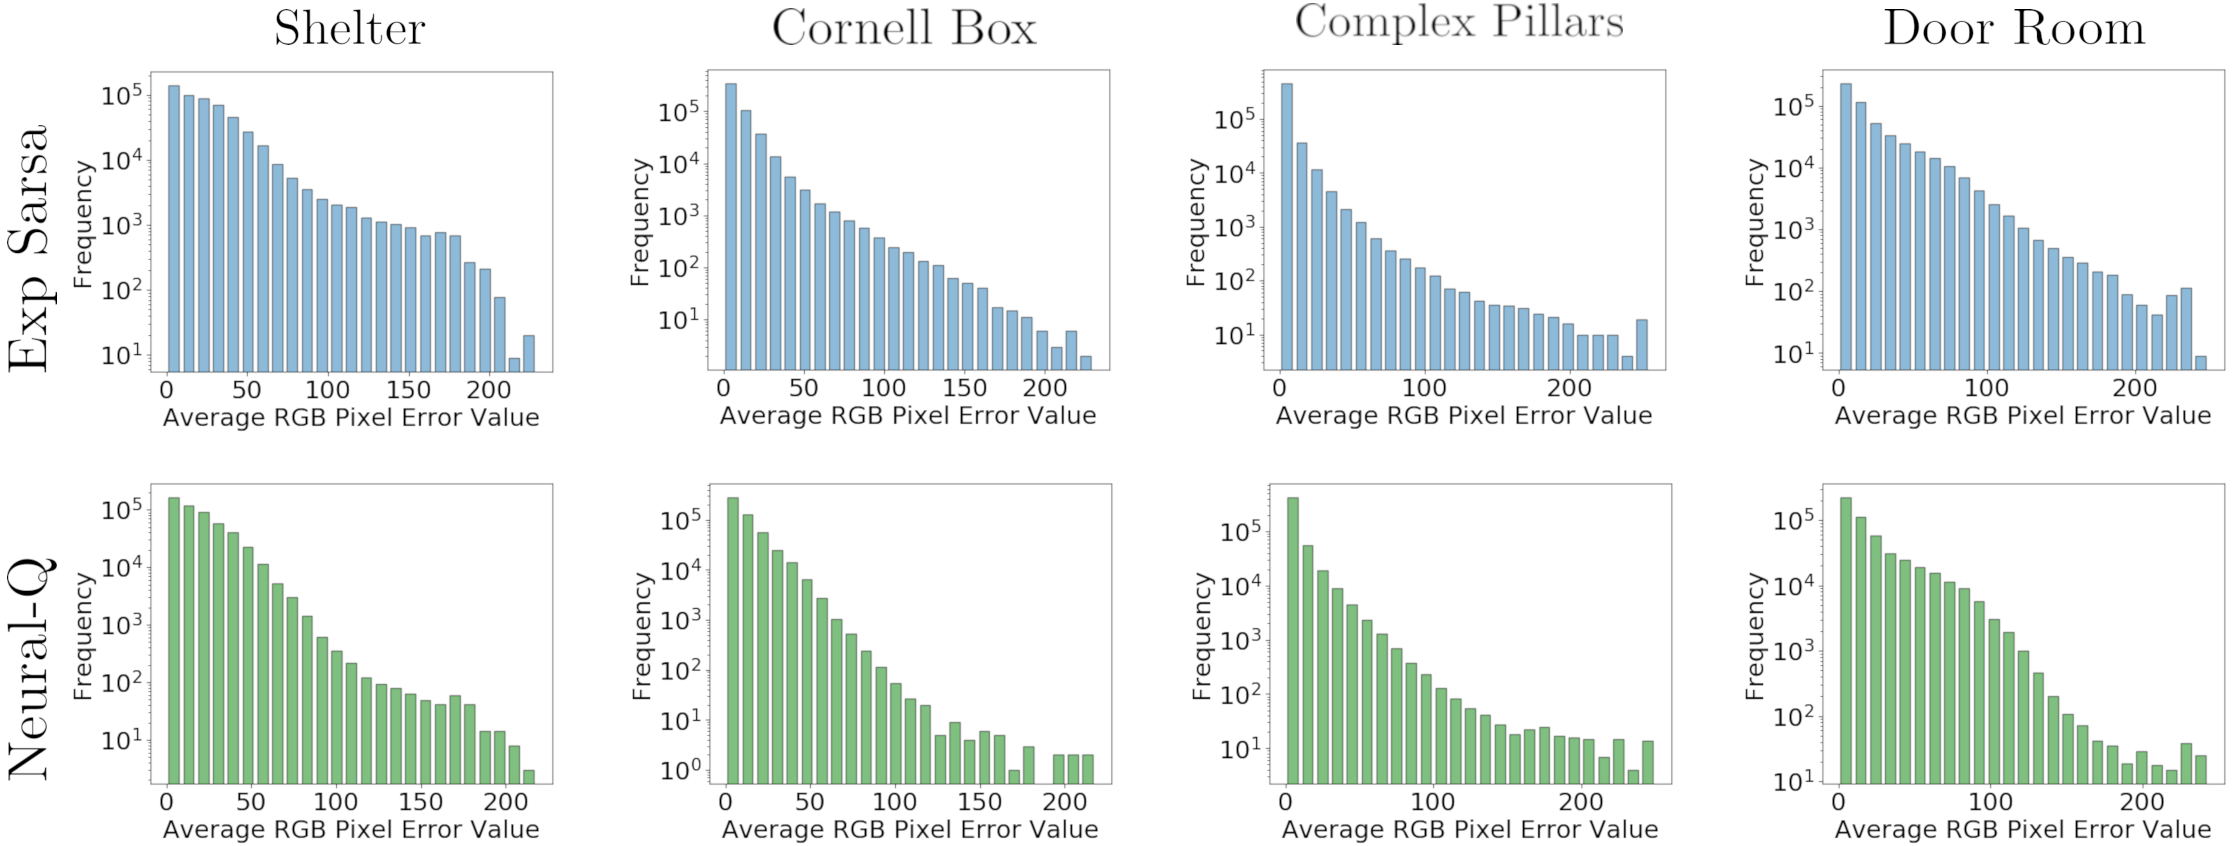
\includegraphics[width=0.99\textwidth]{images/noise_diff.png}    
\end{center}
\caption{Histograms for the average RGB pixel error values for all four rendered scenes using both the Expected Sarsa path tracer and the Neural-Q path tracer. Where the average RGB pixel error value is the average difference in all RGB colour channels between a pixel in the reference image, and the corresponding pixel in the image rendered by either the Expected Sarsa or Neural-Q path tracers. The max average RGB pixel error value is $255$, which corresponds to the case where the reference images pixels value was $(255,255,255)$ whereas the rendered images was $(0,0,0)$ or vice versa. The histograms are based on the rendered images presented in Figure \ref{fig:mape_results_grid}.}
\label{fig:histogram_errors}
\end{figure}

By comparing the tail end of the two rows of histograms, the reasoning behind the fireflies within the Expected Sarsa renders becomes clear. That is, the number of high average RGB error pixels is greater for the Expected Sarsa path tracer compared to the Neural-Q path tracer, which are the direct cause of fireflies. This validates the visual observation of fireflies in the renders shown in \ref{fig:mape_results_grid}. For example, the Door Room scene render from the Expected Sarsa path tracer has many bright white and red pixels compared to the reference images, which corresponds to the high number of the large error values within the histogram. The question now is, why are there more pixels with high error values in the Expected Sarsa path tracer renders compared to those produced by Neural-Q? To answer this question, first recall from section \ref{sec:importance_smapling} the closer the probability density function ($pdf$) comes to normalizing the function being integrated($f(x)$), the lower the variance in the Monte Carlo integral approximation. However, if the probability density function used has a different shape to the function, it can actually increase the variance in the Monte Carlo approximation, as illustrated in Figure \ref{fig:improtance_incorrect}. To relate this concept to learning the incident radiance $L_i(x, \omega)$ for importance sampling in Monte Carlo path tracing, if the error in the approximated incident radiance $L_i(x, \omega)$ is high for a scene, the noise in the approximated pixel values will be higher. This is because a normalised version of $L_i(x, \omega)$ for the light paths intersection point $x$ is used to importance sample a direction to continue a light path in. Therefore, a comparison needs to be made about the difference between the learned incident radiance function between the Neural-Q and Expected Sarsa path tracers to understand why their pixel error values are different.

\begin{figure}[h]
\centering
\minipage{0.45\textwidth}
  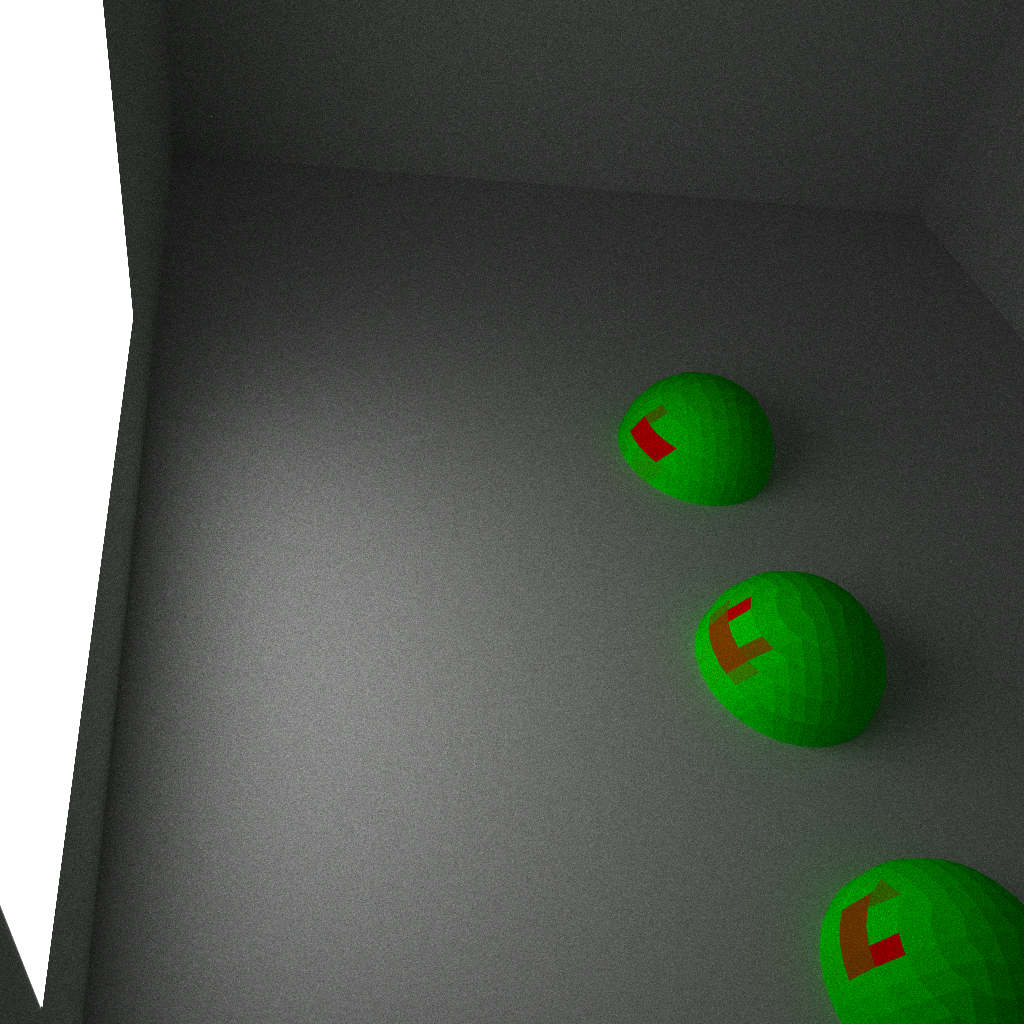
\includegraphics[width=\textwidth]{images/renders/expected_sarsa_visualisation.png}   
  \subcaption{Expected Sarsa}\label{fig:exp_saras_distribution}
\endminipage\hspace{2em}
\minipage{0.45\textwidth}
  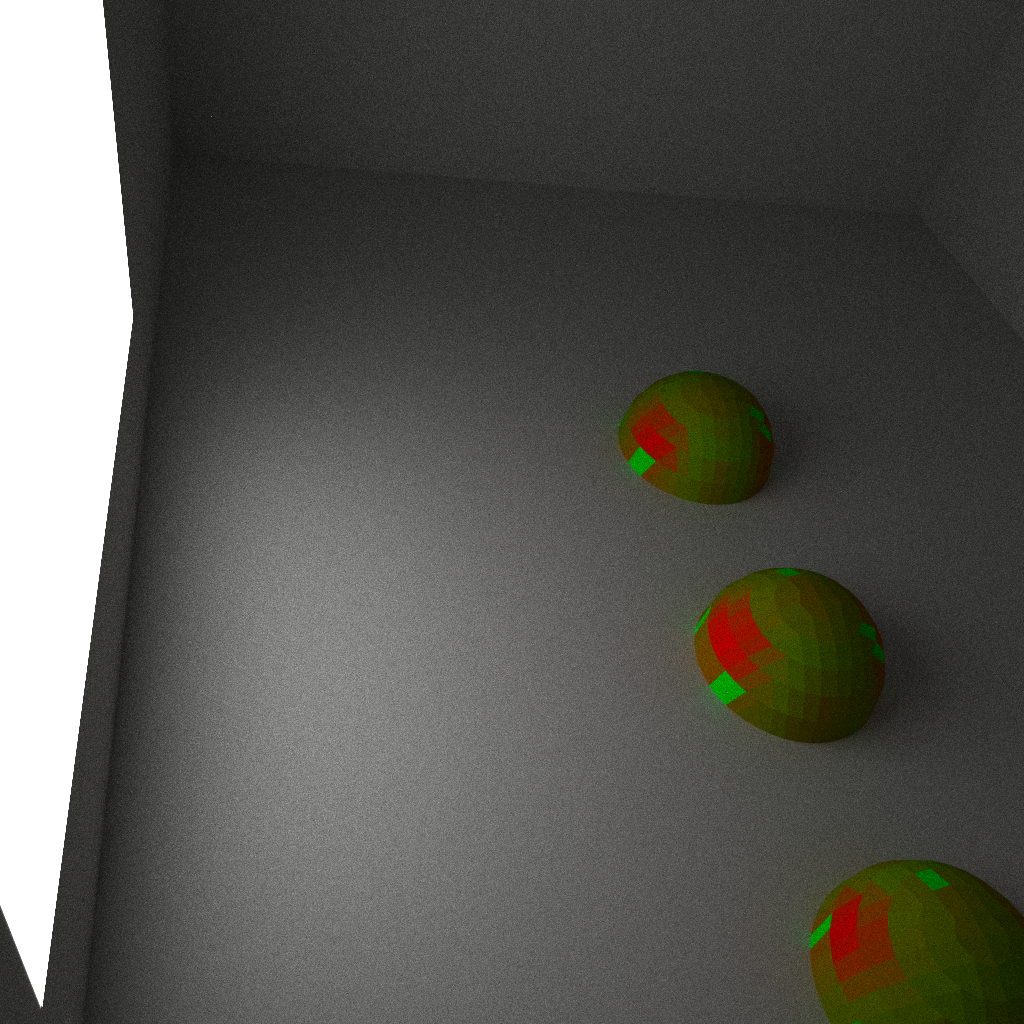
\includegraphics[width=\textwidth]{images/renders/neural_q_visualisation.png}
  \subcaption{Neural-Q}\label{fig:neural_q_distribution}
\endminipage
\caption{Visualisation of the incident radiance at three different points within a scene using both the Expected Sarsa and Neural-Q learned incident radiance function. The learned incident radiance is represented by placing an adaptive quadrature at the point with 144 different sectors, each representing an incident direction which the incident radiance has been estimated at. Sectors where the approximated incident from radiance is at its highest are the sectors which the closest to being red, whereas sectors closer to green have a low incident radiance estimate. The scene consists of a large area light on the left, therefore the large majority of light contributed to a point in the scene are directions which intersect with this light.}
\label{fig:distribution_visualisation}
\end{figure}

As previously explained incident radiance function $L_i(x, \omega)$ is a 5-dimensional function as $x \in \mathbb{R}^3$, $\omega \in \mathbb{R}^2$, making it difficult to visualize. Therefore, in Figure \ref{fig:distribution_visualisation} a visual representation of both the Expected Sarsa and Neural-Q algorithms learned incident radiance for three points in a scene are given. The scene is simple, it has no light blockers and there is a single area light from which the majority of incident radiance on the three points comes from, meaning it clearly presents the differences in the shape of the distribution formed by normalising the incident radiance values at at a point. The Neural-Q incident radiance in Figure \ref{fig:neural_q_distribution} is a far smoother approximation of incident radiance on all three points, compared to that of the Expected Sarsa in Figure \ref{fig:exp_saras_distribution}, due to the spread of sectors with a high incident radiance estimate (red sectors). By observing the relative position of the light in the scene, the Neural-Q's smoother incident radiance estimate is clearly a more accurate approximation, as in the Expected Sarsa quadratures there are many incident angles which lead to a direct intersection with the area light which show a low approximated incident radiance. 

\begin{figure}[!htb]
\centering
\minipage{0.33\textwidth}
\begin{tikzpicture}
	\begin{axis}[every axis plot post/.append style={
	  mark=none,domain=-2:3,samples=50,smooth},
	  axis lines = left,
	  tick style={draw=none},
	  xticklabels={},
	  yticklabels={},
	    % All plots: from -2:2, 50 samples, smooth, no marks
	  axis x line*=bottom, % no box around the plot, only x and y axis
	  axis y line*=left, % the * suppresses the arrow tips
	  enlargelimits=upper,
	  xlabel = $\omega_i$,
	  ylabel = $p(\omega_i)$
	  ] % extend the axes a bit to the right and top
	  \addplot [
	  color=red,
	  ]{gauss(0.5,0.8)};
	  \addplot [
	  color=blue,
	  ]{gauss(0.5,0.5)};
	\end{axis}
\end{tikzpicture}
  \subcaption{Expected Sarsa}\label{fig:dist_expected_sarsa}
\endminipage
\minipage{0.33\textwidth}
    \begin{tikzpicture}
	\begin{axis}[every axis plot post/.append style={
	  mark=none,domain=-2:3,samples=50,smooth},
	  axis lines = left,
	  tick style={draw=none},
	  xticklabels={},
	  yticklabels={},
	    % All plots: from -2:2, 50 samples, smooth, no marks
	  axis x line*=bottom, % no box around the plot, only x and y axis
	  axis y line*=left, % the * suppresses the arrow tips
	  enlargelimits=upper,
	  xlabel = $\omega_i$,
	  ylabel = $p(\omega_i)$
	  ] % extend the axes a bit to the right and top
	  \addplot [
	  color=red,
	  ]{gauss(0.5,0.8)};
	  \addplot [
	  color=blue,
	  ]{gauss(0.5,1.0)};
	\end{axis}
	\end{tikzpicture}  
   \subcaption{Neural-Q}\label{fig:dist_neural_q}
\endminipage
\caption{An illustration of the incident radiance distribution for a given point directly in front of the light source shown in Figure \ref{fig:distribution_visualisation} for both the Expected Sarsa and Neural-Q methods. Where $\omega_i \in \Omega$ is discrete incident angles on the point, and  $p(\omega_i)$ is the probability density function over incident radiance evaluated at angle $\omega_i$. The \textbf{red} line represents the true incident radiance distribution on the point, the \textbf{blue} represents a smoothed version of the corresponding methods approximation of the incident radiance distribution on the point.}
\label{fig:dist_2_methods}
\end{figure}


To give a better a conceptual understanding of why Expected Sarsa is less accurate compared to Neural-Q for the setting in \ref{fig:distribution_visualisation}, an illustration of in Figure \ref{fig:dist_2_methods} of an example incident radiance distribution for an intersection point in front of the area light is given. Whereby normalising the incidence radiance prediction over all angles in a hemisphere $\Omega$ around an intersection point, a probability density function over the predicted incident radiance on the intersection point is formed. The probability distribution for the Expected Sarsa approach is leptokurtic, meaning it contains an excess of extreme values causing it to incorrectly model the true incident radiance distribution for a point in the scene. Whereas the more mesokurtic curve for the Neural-Q path tracer more accurately models the true underlying incident radiance distribution, however it is not perfect hence the noise still present in rendered image. Note, this This inaccuracy by Expected Sarsa means for some incident angle $\omega_i$ which is not on the peak of the approximated distribution will likely have a significantly lower contribution of radiance to a point $x$ then it actually provides. Meaning, the probability density function $pdf(x, \omega_i)$ will be small, and when used to divide the numerator in Equation \ref{eq:rendering_eq_monte_carlo}, the approximated pixel colour value will be much higher then its true value. This ultimately leads to the 'fireflies' noise in the rendered images for the Expected Sarsa approach in Figure \ref{fig:mape_results_grid}. In \cite{dahm2017learning} it is suggested that Expected Sarsa algorithm does not necessarily converge on the incident radiance, which is exactly what has been shown in \ref{fig:distribution_visualisation}.

\section{Convergence}
\label{sec:convergence_learning_incident}

Another important property which has not yet been discussed is the number of SPP required for the Expected Sarsa and Neural-Q algorithms to convergence on their approximation of the incident radiance function $L_i(x, \omega)$. To assess this, the number of zero contribution light paths when rendering a single image has been , as well as the average number of reflections a light path undergoes before intersecting with a light source, known as the average path length are both plotted against accumlated rendered images using 1 SPP (Epoch). For a scene where a light path is guaranteed to intersect with an area light (sealed scene), as the average path length reduces, the number of zero contribution light paths also decreases. This is due to light paths with a shorter length generally contribute more to the rendered image because of the rendering equation. Following importance sampling for Monte Carlo integration, the lower the number of zero contribution light paths sampled in path tracing, the lower the image noise \cite{dahm2017learning}.  This is shown in Figure \ref{fig:training_curves_archway} where the average path length curves correlate with the number zero contribution light paths across accumulated frames for the Shelter scene. Leading to a reduction in noise from first rendered image to the 100th rendered images for both algorithms using 1 SPP to render each image. Note, a similar pattern was seen for the Cornell Box, Complex Pillars, and Door Room scenes.

\begin{figure}[h]
\begin{center}
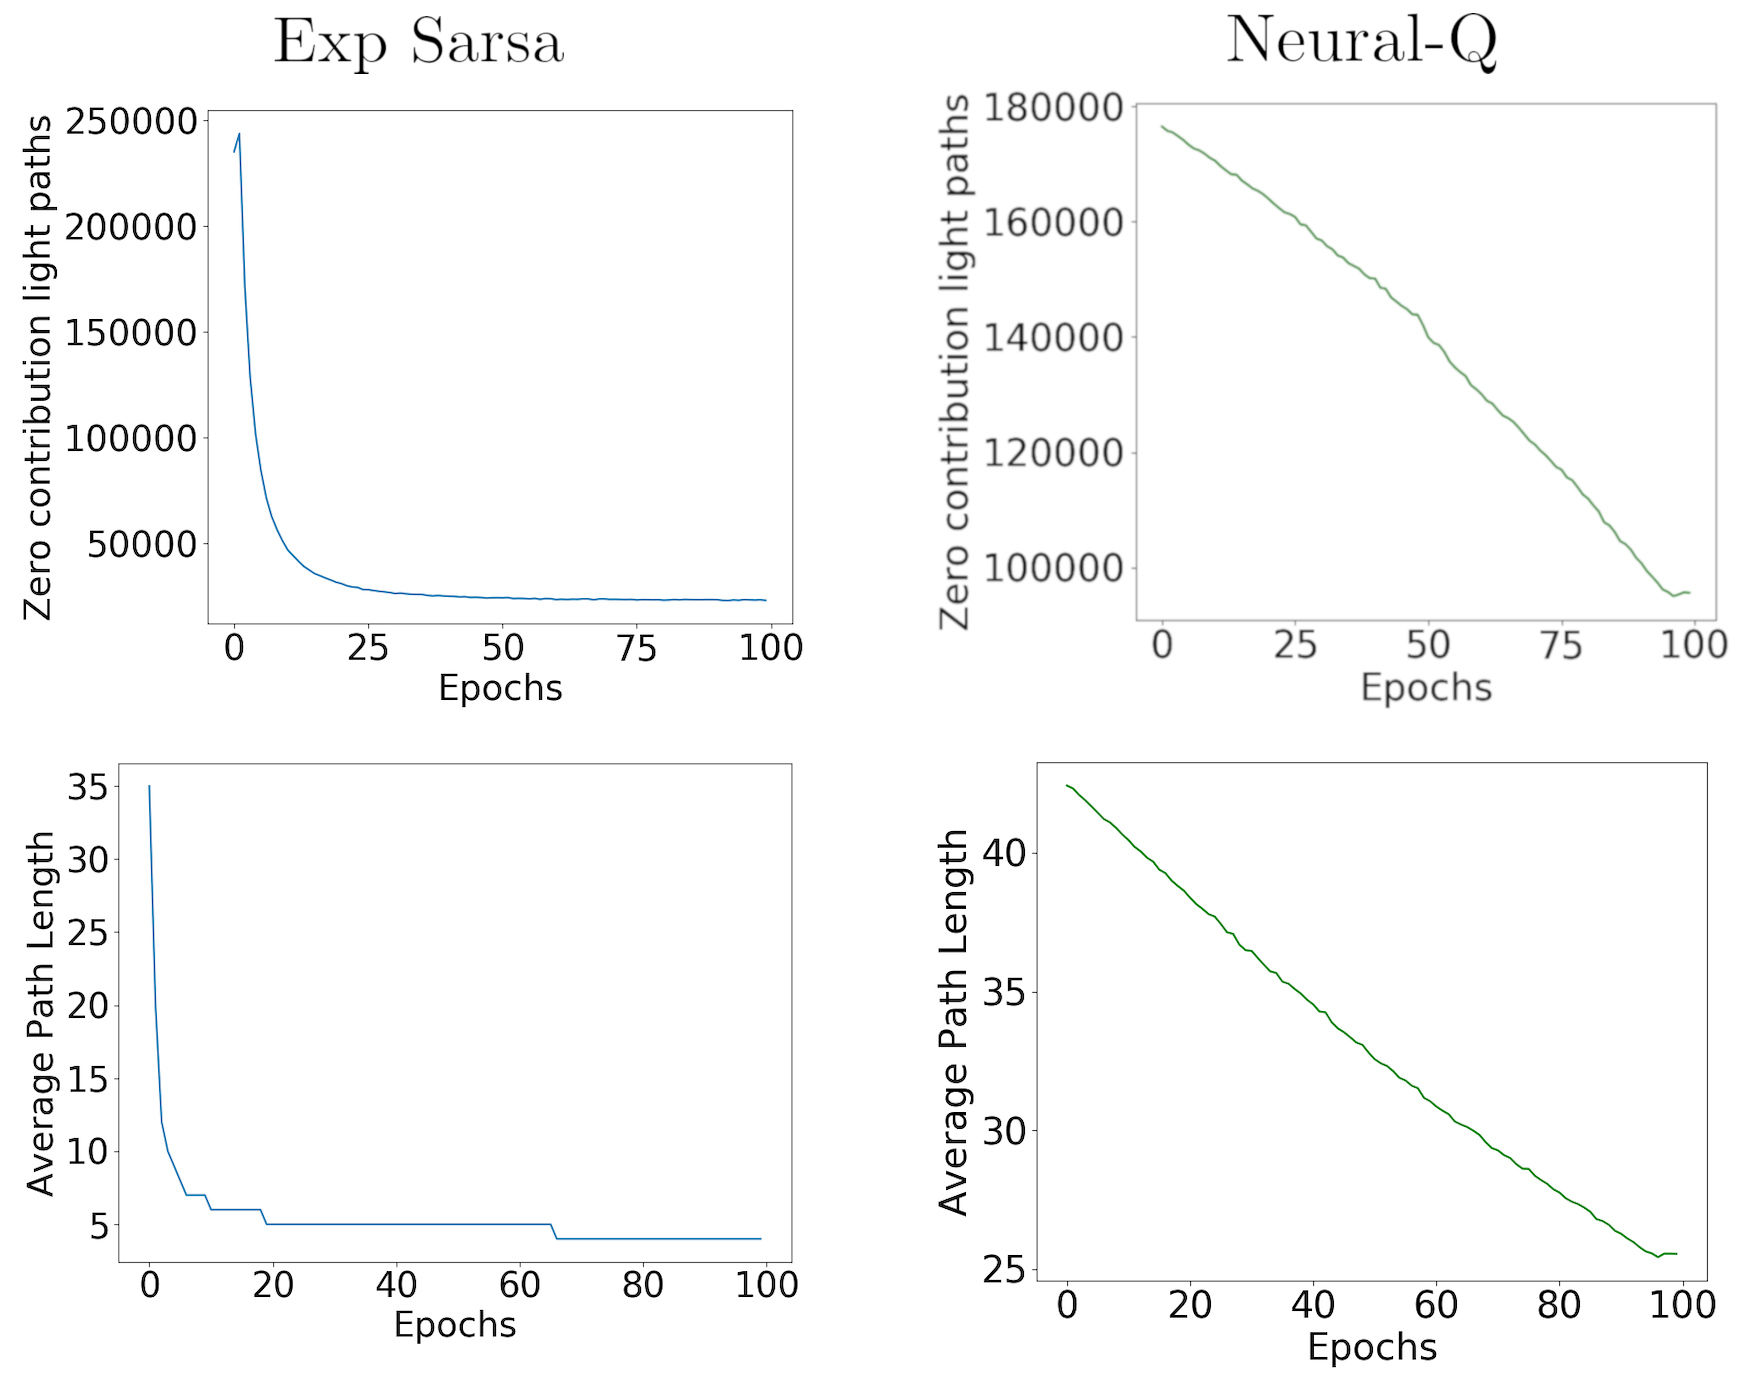
\includegraphics[width=\textwidth]{images/training_curves.png}    
\end{center}
\caption{Training curves for the average path length and number of zero contribution light paths when rendering the Shelter scene for 100 epochs, as well as the 1st and 100th rendered frame when using 1 SPP for both images. This is shown for both the Expected Sarsa and Neural-Q path tracers. An epoch represents one sampled light ray through every pixel in the image. The average path length is the number reflections a light path takes before intersecting with a light source. A zero contribution light path is one which contributes almost zero colour to the final image.}
\label{fig:training_curves_archway}
\end{figure}

An interesting observation is how both the number of zero contribution light paths and the average path length for the Expected Sarsa algorithm fall far below that of the Neural-Q algorithm , yet the MAPE score for the Archway scene is significantly higher for Expected Sarsa in \ref{fig:mape_results_grid}. This leads to the conclusion that the Expected Sarsa path tracer has the potential to further reduce the number of zero contribution light paths compared to the Neural-Q path tracer. However, this alone does not directly reduce image noise. Recall from the previous section \ref{sec:close_inspec_pixels} the leptokurtic shape of the incident radiance distribution approximated by the Expected Sarsa method for a given point in the room does not accurately describe the true underlying radiance distribution. Therefore, the probability density function used to normalise the Monte Carlo prediction of a light paths colour estimate adds fireflies noise to regions of the image.\\

By observing the curves for the number of zero contribution light paths and average path length for both methods in \ref{fig:training_curves_archway}, it is clear that the Expected Sarsa approach is able to more quickly learn the incident radiance function $L_i(x, \omega)$ compared to the Neural-Q path tracer. However, the almost linear decrease seen for both curves using the Neural-Q method is due to the use of an $\epsilon$-\textit{greedy} policy. As previously described in section \ref{sec:ann_architecture}, the $\epsilon$-\textit{greedy} policy ensures the Neural-Q algorithm initially prioritises exploration ($\epsilon$ is high) to find the approximate value of $L_i(x,\omega)$ by uniformly at random sampling directions to continue light paths in. Every time all pixels in the image have had a light path sampled through them, the value of $\epsilon$ is decayed to favour exploitation more and more. This causes the Neural-Q path tracer to importance light path directions over using its current estimate of $L_i(x, \omega)$. As the decay was set to $\delta = 0.05$ and initially $\epsilon = 1$, the Neural-Q path tracer is limited to just randomly sampling directions to continue light paths in, but it gradually favours importance sampling directions which are more likely to lead to a light source over time. This causes this close to linear downwards trend for the average path length and number of zero contribution light paths, as $\epsilon$ is decreased linearly. 

%TODO image without epsilon greedy strategy for NN and learning rates


As shown in \ref{fig:no_epsilon_greedy}, without a decaying $\epsilon$-\text{greedy} policy where $\epsilon = 0.05$ the Neural-Q algorithm performs worse then without a decaying $\epsilon$-\text{greedy} policy. This is to be expected as there is no exploration prioritisation at the start of its learning, so the algorithm does not discover more optimal directions to sample light rays in over the long term.

\section{From a Discrete to Continuous State Space}

%TODO sarsa's prediction of the incident radiance is discretized, this needs to go in technical with the $Qx_m, \omega_k)$ and capital K for Neural-Q directions
As a reminder, a state in the context of Neural-Q learning is an intersection location $x$ within the scene of a light path. An action is choosing a direction to continue the light path in from the intersection point. As discussed in section \ref{sec:deep_rl_motivation}, the Neural-Q algorithm uses an ANN as a function approximator for learning the incident radiance function ($L_i(x, \omega)$) where the approximation is denoted as $\hat{q_\theta}(x, \omega_k)$ for the discrete set of actions $\forall k = 1, ..., K$, over the continuous space of intersection positions $x \in \mathbb{R}^3$. Whereas Expected Sarsa uses a tabular approach denoted as $Q(x_m, \omega_k)$,  $\forall m = 1, ..., M$ discrete intersection locations in the scene, $\forall k = 1, ..., K$ discrete set of actions. Therefore, as the the approximation of $L_i(x, \omega)$ by Neural-Q is made by an ANN, to find the estimated incident radiance for an unseen intersection location $x' \in \mathbb{R}^3$ in direction $\omega_k$, the ANN can use its current parameter values $\theta$  to generalize the incident radiance $\hat{q_theta}(x', \omega_k) \sim L_i(x', \omega_k)$. Whereas the approach of Expected Sarsa is to find the closest Irradiance Volume to the point located at $\bar{x}$ and use its stored incident radiance estimate for the approximation, that is $Q(\bar{x}, \omega_k) \sim L_i(x', \omega_k)$. 

\begin{figure}[h]
\centering
\includegraphics[width=\textwidth]{images/1_spp.png}   
\caption{Reference Images of the The Door Room and Shelter scenes next to SPP renderusing both na trained Expected Sarsa path tracer, and a trained Neural-Q path tracer trained for 100 epochs. The single sample for each pixel in the Expected Sarsa and Neural-Q renders is constructed by reflecting the light path in the direction of highest estimated radiance upon every intersection point, until the light is intersected with.}
\label{fig:1_spp_max_dir}
\end{figure}

The benefit in memory usage is discussed in detail within section \ref{sec:mem_to_comp}. Here however, I will present how the generalization for unseen intersection locations allows the ANN to learn a smooth approximation of the incident radiance for any point in the scene, compared to the Expected Sarsa method. Observe Figure \ref{fig:1_spp_max_dir}. As stated, a single light path is sampled through each pixel using the three different path tracing algorithms discussed. The difference is that the trained Expected Sarsa and Neural-Q path tracers sample the ray at any intersection point in the direction of maximum predicted radiance. Therefore, the goal of \ref{fig:1_spp_max_dir} is to not reduce image noise in the renders of the two scenes at 1 SPP for both methods, but to instead visualize for any point in the scene the largest amount of incident radiance on any given point in the scene. This uncovers the differences in the approximation of the incident radiance for any given location in the scene between the Expected Sarsa and Neural-Q path tracers.\\

For both renders shown in \ref{fig:1_spp_max_dir} produced by the trained Expected Sarsa path tracer there are small distinct darker regions of the image. Each one of these small dark regions represents an Irradiance Volume which has not converged on a direction to sample in which leads to a high contribution of incident radiance. This creates small distinct areas where the estimation of incident radiance is poor, which is likely to lead to higher levels on image noise in these locations when they are intersected with during path tracing. On the other hand, a vastly different pattern can be seen for the Neural-Q algorithms renders, where boundaries between regions with a better approximation for the highest incident radiance direction are much smoother then that of the Expected Sarsa's. This is due to the generalization for incident radiance over the unseen states, where no longer discrete incident radiance values are stored, but instead the parameter values $\theta$ of the network determine an arbitrary decision boundary in the 5D space for predicting $L_i(x, \omega)$.\\

The question now is, does the generalisation over the state space made by Neural-Q actually help to reduce image noise compared to the discretized approach by Expected Sarsa? Unfortunately there is no clear answer to this question from the data I have collected. The reason being, the ANN generalization improves the approximation of $L_i(x, \omega)$ in both  the Shelter and Complex Pillars scenes, whereas it performs equally for the Door Room scene and worse for the Cornell scene. So at best I can conclude the ANN generalization can be more  beneficial for scenes with larger and more complex geometry whilst using less memory \ref{sec:mem_to_comp}. This is represented  in \ref{fig:1_spp_max_dir}, where on average for the Neural-Q's render of the Shelter scene, the direction of highest incident radiance is accurately learned. Whereas there are far more dark patches  in the Expected Sarsa's render which represent incorrect approximations of the optimal direction to sample in. However, for smaller less complex scenes (Cornell and Door Room scenes) the ANN's approximation quality of incident radiance heavily changes across neighbouring regions in the scene. As a result, Figure \ref{fig:mape_results_grid} shows Neural-Q's performance against the Expected Sarsa approach is slightly worse for reducing image noise. In order to remedy the ANN's poor approximation in such situations, modifications in the ANN's architecture may be required. But this seems to be part of a wider problem which comes with a lack of research into how ANN architecture affects the quality of the approximated incident radiance function $L_i(x, \omega)$ for various types of scenes, which requires more research before ANN's can be stably used to importance sample light paths in Monte Carlo path tracing to reduce image noise for any arbitrary scene. Some progress has been made in this very recently, which I will discuss later in section \ref{sec:recent_advancements}.

\section{From Memory Bound to Compute Bound}
\label{sec:mem_to_comp}

Computational resources utilized by the path tracing algorithms introduced is a very important talking point when considering the potential to be integrated into renders used in industry such as \cite{georgiev2018arnold, christensen2018renderman, hyperion}. In particular any bounds imposed on the algorithm from current available hardware are the most important to consider, as rendering algorithms should be designed to give as much power to artists as possible to create and render any arbitrary scene of their choice. A detailed investigation on both highly optimised implementations of the Expected Sarsa and Neural-Q path tracers performance using current available hardware warrants a detailed investigation in itself. Instead for completeness, this section presents a high level analysis of how both memory usage and compute power limits their performance.

\subsection{Memory Usage}

The default forward path tracer is compute bound, meaning the only way to make the algorithm faster is by providing more compute power. For example by parallelizing the rendering process using a GPU with a quicker processor clock speed. On the other hand, the performance of the Expected Sarsa algorithm for reducing image noise has been found to be bound by the amount of RAM the algorithm has available to it from the  underlying hardware. This is due to the requirement of storing the Q-table in RAM which holds the approximated incident radiance values for a scene.\\

\begin{table}[h]
	\centering
	\begin{tabular}{lcc}
		\toprule
		& \multicolumn{2}{c}{Memory (MB)} \\ \cmidrule(lr){2-3}
		Scene & Expected Sarsa & Neural-Q \\
		\midrule
		Shelter & 271 & 30 \\
		Cornell Box & 44 & 30 \\
		Complex Pillars & 300 & 30 \\
		Door Room & 66 & 30 \\
		\bottomrule
	\end{tabular}
	\caption{Additional memory required in Megabytes (MB) to render each of the four scenes shown in Figure \ref{fig:mape_results_grid} using both the Expected Sarsa and Neural-Q path tracers.}
	\label{tab:memory_usage}
\end{table}

\subsubsection{Expected Sarsa}

The size of memory used by the Q-table is defined by the number of Irradiance Volumes sampled across the scenes geometry, as well as the number incident radiance values stored for directions $\omega_k$ $\forall k = 1,...,n$  within each Irradiance Volume. I have found the higher the number of sampled Irradiance Volumes the more accurate the incident radiance approximation is for a given intersection point, as shown in Figure \ref{fig:more_irradiance_volumes}.  Intuitively this makes sense, as for the incident radiance function $L_i(x, \omega)$, the position $x \in \mathbb{R}$ can be infinitely many positions  in the scene. Therefore, the more Irradiance Volumes used to store approximated incident radiance values, the closer the approximation will be to the true function. In terms of the algorithm, the average distance from a light path intersection point to the closest Irradiance Volume decreases as the number of Irradiance Volumes sampled in the scene increases. This becomes clear by observing Figure \ref{fig:voronoi_difference}, where the Voronoi plot of the scene with a lower number of sampled Irradiance Volumes on average has a larger sector size. Meaning, on average the nearest neighbour search will return an Irradiance Volume further away from the intersection point compared to when more Irradiance Volumes are sampled. Recall that a nearest neighbour search is used to estimate the incident radiance on a point based on the stored values in the closest Irradiance Volume, therefore the closer the Irradiance Volume used for this approximation the more accurate the approximation of incident radiance on the point will be.\\

% 1 image for more irradiance volumes leading to higher MAPE score -> showing the scene discretization

    


A clear problem from this relationship is that if the underlying system does not have enough RAM, then the algorithm will not be able to significantly reduce the amount of noise in rendered images. Now, this may not be a problem for most small scenes with a polygon count ofaround 100, as common commodity graphics cards such as the NVIDIA 1070Ti GPU used for my experiments comes with 8GB of global memory (RAM), and NVIDIA claim they are able to fit the Q-table for a such scenes into only 2MB of memory to receive a significant reduction in noise \cite{dahm2017learning}. However, films commonly render scenes with hundred of thousands, or even millions of polygons potentially making it impossible to store a Q-table large enough to significantly reduce image noise in RAM. For example, in Transformers Revenge of the Fallen, the robot 'Devastator' was made out of 11,716,127 polygons \cite{devastator}. To present this memory scaling issue, Figure \ref{} presents a render of the Cornell Box scene which uses only xMB of memory to store the Q-table. The artefacts present in the image are cause by vastly incorrect importance\\

%1 image showing artefacts from too low number of irradiance volumes

\subsubsection{Neural-Q}

The Neural-Q path tracer on the other hand does not have exhibit the scaling in memory requirements as that of the Expected Sarsa path tracer. The is due to the Neural-Q path tracer only requiring more memory to store the incident radiance values for the current batch of light paths, which are used to importance sample directions for continuing the batch of light paths in. As well as, the amount of RAM required to store the ANN. The memory required to store the current batch of incident radiance values is controllable by the batch size parameter for the number of rays, therefore does not scale with the complexity of the scenes geometry. But a study from \cite{ren2013global} suggests more layers may be required in ANNs to approximate the incident radiance $L_i(x, \omega)$ for scenes with more complex geometry, meaning more memory is required to store more weight parameters of the network. However, further experimentation must be done to investigate the scaling of memory usage to scenes with thousands of vertices for the two rendering methods, by using a more optimised rendering engine then the one I have built. The renders presented in Figure \ref{fig:mape_results_grid} were produced using a constant ANN architecture as specified in \ref{sec:ann_architecture}, which required only 30MB of memory to store the ANN as well as intermediate values computed during a forward pass. Whilst the Expected Sarsa path tracer required the rendered scenes with different geometry to have significantly different Q-table sizes to reduce rendered image noise. This is due to the ANNs ability to generalize the approximated incident radiance over the 5D space formed by a position $x \in \mathbb{R}^3$ and direction $\omega \in \mathbb{R}^2$. Where a single weight in the ANN has the capacity to contribute to the approximated radiance of many positions and directions in the scene. Hence, an ANN with 2 hidden layers was able to make a good approximation of the incident radiance for any $(x, \omega)$ for all tested scenes. The Q-table on the other hand holds an individual value for each incident radiance estimate $(x,\omega)$, therefore the storage requirements rose for the scenes rendered with more complex geometry. For example, the Q-table required for the Expected Sarsa rendering of the large archway scene without any artefacts used 272MB of data storage, 9X more than that of the Neural-Q path tracer.


%TODO number of sectors in irradiance volumes and its effect
%Moreover, the higher the number of discrete directions$n$ held in each Irradiance Volume, the more accurate the estimated radiance distribution at the given intersection point will be, see Figure \ref{fig:more_directions}. This is because the true radiance distribution at any point in the scene is continuous, so the more samples used in the Monte Carlo approximation of this probability density function (see section \ref{sec:td_light_transport}), the lower the approximation error due the law of large number in Equation \ref{eq:law_large_numbers}. 

\subsection{Parallel Processing}

For high quality, high frame rate rendering of scenes, rendering algorithms in general become very computationally demanding \cite{crockett1995parallel}. In order to facilitate this high level of performance, parallel computing must be used to distribute the computational workload. This pattern follows for both scanline renderers and ray-tracing renderers (which path tracing falls into) \cite{alerstam2008parallel, fatahalian2009data}. The default path tracing algorithm in particular is an embarrassingly parallel algorithm \cite{embarissingly_parallelizable}, as the task of finding the colour estimate of a single light path can be performed independently by a single process without any communication to other processes. A simple example of this is given in \cite{accelerated_ray_tracing}, whereby using GPU the process of rendering an image using an algorithm which closely resembles path tracing is split among many cores on a GPU. In industry path tracing algorithms take advantage of parallelism to an unprecedented scale, such as Disney's supercomputer for rendering full-length films using the Hyperion renderer \cite{hyperion}. Therefore, for any modified path tracing algorithm to gain industries attention it needs to be able to take fully advantage of parallel computing hardware.\\

\subsubsection{Expected Sarsa}

The Expected Sarsa path tracer is no longer as trivial to parallelize as the default forward path tracing algorithm due to the the first addition to the algorithm detailed in section \ref{sec:expected_sarsa_path_tracer}, where the incident radiance estimate for a given entry $Q(x,\omega_k)$ is updated after each intersection point is traced for constructing a light path. To parallelize the algorithm means to create and individual process to construct each light path as part of determining the estimate of a pixel value. However, the Q-table which stores the current approximation of all discrete incident radiance values in the scene is accessed by each thread. Meaning, it is possible that two threads will attempt to write to the same location at the same time in the Q-table if they intersect near one another, causing the update rule provided in Equation \ref{eq:mc_expected_sarsa_td_learning} will not be applied correctly. To remedy this, the update rule can be placed within a critical code section \cite{raynal2012concurrent} to ensure only one thread at a time can calculate and set the updated incident radiance estimate. For my purposes, all code written for parallel execution used the CUDA Toolkit \cite{cuda}, where CUDA atomic operations were used to ensure only one thread at a time can calculate and apply the Q-value update. The critical section added a minor performance overhead to each thread in both waiting to and performing the update rule. However it was negligible when using a Q-table near the size of any used to render the images in \ref{fig:mape_results_grid}, as due to the number of Q-values it is rare two threads attempt to write to the same address at the same time.\\ 

A significant performance penalty I found the Expected Sarsa method imposes on path tracing, is the time taken to perform the nearest neighbour search for finding the closest Irradiance Volume to a given intersection point in the scene. Whilst I implemented a KD-Tree on the GPU in order to reduce the nearest neighbour computational complexity to $O( \log n)$, I found the Expected Sarsa path tracer ran XX times slower then that of the default path tracer. The cause of this slowdown was found to be in per thread memory read times to global CUDA memory \cite{cuda_c_guide}. As a quick overview of CUDA's thread hierarchy; an execution thread in CUDA is contained within a group of threads known as a thread block. Each thread block is executed by a symmetric multiprocessor (SM) placed in a GRID. Following this, the memory hierarchy consists of per-thread local memory, per-block shared memory, and global memory which any thread can read and write to at any time. The issue with the Expected Sarsa path tracer is the Q-table is that the Q-table needs to be globally accessible to any thread in the GPU at any time, as every thread will be constructing a light path and during its construction it may update the value of any $Q(x, \omega)$ in the Q-table. This compounded with that the Q-table is far too large to store in per-thread or per-block memory for any commodity GPU, means nearest neighbour lookup performs $O(\log n)$ global memory lookups. Each uncached global memory lookup has roughly 100X higher latency then that of per-thread or per-block memory lookups \cite{global_vs_shared}. Hence, the Expected Sarsa algorithm experiences a high performance penalty from idle time waiting for data to be returned from global memory. Note, NVIDIA claims that the Expected Sarsa path tracer is able to render images with the same number of samples per pixel only 20\% then that of the default path tracer \cite{dahm2017learning} to significantly reduce image noise, however they do not specify the details of the machines that were running these experiments. My implementation could be further optimised by ensuring aligned memory access and reducing the amount of data retrieved, however it is unlikely that any of these optimisations will be able to avoid the bottleneck of regularly querying global memory.\\

\subsubsection{Neural-Q}

%TODO timing stats for training and tracing rays -> compared to expected sarsa as well
As for the Neural-Q path tracer parallel execution is slightly different, whereby batches of light paths colour estimates are computed once at a time. Note, the batch size should be set to be large enough such that no processors are idle whilst computing a batch, whilst being able to hold the temporary approximated incident radiance values in memory which are used for importance sampling directions to continue light paths in. Also, mini-batches which are the same size as the batch of light paths can be used in querying and training the ANN by stochastic gradient descent. A problem which added a significant performance penalty on my approach compared to that in \cite{muller2018neural}, is that there was no built in way to evaluate an ANN per-thread on the GPU using the Dynet framework, only code from the CPU could call any of the Dynet API functions. Meaning, my implementation had to frequently send data produced from tracing a batch of light paths to their next intersection point (positions, normals, throughputs etcetera) from the GPU to the CPU, only to call a dynet function which moved the data back to the GPU again for evaluating the ANN. Within Algorithm \cite{alg:neural_q_path_tracer} there are a total of $3$ calls to the Dynet API for evaluating the network for every batch of light ray paths, this means there is a total $6$ batch data transfers from the host device memory (that directly accessible by the CPU) to GPU memory, as illustrated in \ref{fig:memory_transfer}. \\

% Illustration of data transfers

The latency added by this design flaw is mainly due to the peak bandwidth available for transferring data between memory in the GPU is 144 GB/s, while for transferring data from the CPU to the GPU (and vice versa) is only 8 GB/s \cite{global_data_transfer}. Therefore, the 18x performance penalty received $6$ times with each batch computation, makes evaluating my implementation of the Neural-Q path tracer on render time not a fair test. However, the performance penalty received by methods which use neural network based importance sampling for Monte Carlo path tracing have found that the cost of the evaluating the ANN without the data transfers from CPU to GPU (and vice verca) can still add a 10X peformance penalty compared to other importance sampling methods in some cases \cite{muller2018neural, keller2019integral}. Clearly this needs to be alleviated before the neural network importance sampling methods are adopted for Monte Carlo path tracing in industry. Answers to this problem may already lie in existing hardware, by leveraging the power of NVIDIAS TensorCores in Tesla GPUs \cite{tensor_cores}, which claims to have 40X higher performance than CPUs for inference on ANNs.


\section{Hyperparameters}

The final point of comparison between the Expected Sarsa and Neural-Q path tracers is the hyperparameters which must be configured for the algorithms. One of the enticing parts of using path tracing in industry is its lack of parameters \cite{georgiev2018arnold}. It turns out a lack of parameters is very important to artists for rendering photo-realistic images of scenes, as they are able to iterate quicker in their development of a scene. For example, when developing a scene for a film, an artist will constantly changing the geometry and will need a rendering algorithm which requires little configuration to quickly render a scene \cite{georgiev2018arnold}.

\subsubsection{Expected Sarsa}
The default path tracing algorithm (Algorithm \ref{alg:default_path_tracer}) only requires the number of SPP to be set for the rendered image. Along with the SPP, the Expected Sarsa path tracer requires the amount of memory to use for the Q-table which is used to approximate the incident radiance function \cite{dahm2017learning}. As described in \ref{sec:mem_to_comp}, the higher the amount of memory given to the algorithm, the more Irradiance Volumes sampled around the scene. This leads to a more accurate approximation of the incident radiance function. Not only does this present the issue that for more complex scenes, more memory is required, but actually determining the minimal amount of memory required to significantly reduce the noise without any artefacts in rendered images is a difficult task. By artefacts, I mean large areas of the image which have a significant amount of noise, such as that seen in \ref{}.\\

 My approach for determining the amount of memory a scene required was to instead determine the number of Irradiance Volumes to sample per-polygon in the scene. This was done by setting a surface area to Irradiance Volume ratio; for example say the ration was $1:10$ every $1 \text{cm}^2$ of surface area in the scene would have 10 Irradiance Volumes sampled upon it. This changes the parameter from arbitrarily guessing the memory required by the scene to a ratio which takes less time to find the optimal value for in practice. However, the trial and error approach required to find the correct value is still present, but just to a lesser degree. Clearly finding the optimal memory usage for the discretization of the scene in the Expected Sarsa method is a time consuming process. In practice, it may take longer to find an optimal amount of memory to render a scene with thousands of vertices without artefacts, than it does to just use the default path tracer with a higher SPP to get rid of noise. Note, this is more of a problem for cases where memory usage is a concern, such as rendering scenes which require many textures to be stored in memory.
 
\subsubsection{Neural-Q}
 The Neural-Q path tracer was shown to significantly reduce the noise in rendered images using a fixed amount of memory for the ANN architecture provided in Figure \ref{fig:mape_results_grid}. Therefore, the parameter for memory provisioned by the algorithm does not need to be specified by the user. However, as discussed in section \ref{sec:mem_to_comp}, the ANN may require more layers to represent scenes with more complex geometry then those I have experimented with. For now, the Neural-Q algorithm only exposes two parameters; the beginning $\epsilon$ value and the decay rate $\delta$ both defining the $\epsilon$-\textit{greedy} policy to follow. It is common practice to begin start with $\epsilon = 1$, as initially the reinforcement learning agent has no prior knowledge of which actions are more valuable to take \cite{mnih2013playing, van2016deep, mnih2015human}. The same goes for the Neural-Q path tracer, as initially the ANN has no knowledge regarding the incident radiance from any given directions, on any points in the scene. Meaning, $\epsilon = 1$ is a simple choice to make. The less trivial parameter is the decay $\delta$ which should be high enough for the algorithm to quickly start exploiting its approximation of the incident radiance function $\hat{q_\theta}(x, \omega_k)$, by importance sampling. Yet low enough, such that the algorithm efficiently builds an accurate estimate of the incident radiance for any point in the room, for any incident direction. The choice of $\delta = 0.05$ for all renders presented in Figure \ref{fig:mape_results_grid} was made as it fit the criteria specified for the four scenes experimented with. This is not to say this is the universal best decay rate for all scenes. It is likely scenes with a large number of blockers and complex geometry require more exploration, however this is something yet to be explored along with Neural-Q in general on scenes with a very large number of polygons in general.\\
 
The Neural-Q algorithm's parameters are clearly easier to configure for rendering an arbitrary scene, compared to the Expected Sarsa's. Having to manually decide on memory usage is no easy task and is far too dependent on the scene being render itself. Meaning, every change to geometry when building a scene using a production path tracer such as \cite{georgiev2018arnold, christensen2018renderman, hyperion} will require the difficult process of estimating the memory needed to render the scene without artefacts. This is something artists would definitely wish to avoid when designing a scene.

\section{Recent Advancements in Neural Importance Sampling for Monte Carlo Path Tracing}
\label{sec:recent_advancements}

%TODO using monte carlo approximation essentially smoothes the neural networks estimate rather then directly approximating the incident radiance 

Along with Nvidia's paper which suggested a reinforcement learning approach for approximating the incident radiance at any point in a scene \cite{dahm2017learning}, other reinforcement learning based methods for learning light transport in a scene have been engineered \cite{muller2017practical, vorba2014line}, but none of them investigated the potential of deep reinforcement learning for this problem. However, recently neural networks for both the global and local sampling for light path construction have had a large amount of research \cite{zheng2018learning, muller2018neural, keller2019integral, hermosilla2018deep}. Global light path sampling is where the optimal density of sampled light rays per pixel is determined by the learning algorithm. Therefore, the reinforcement learning agent only determines where light paths should initially be sampled from. While this method does not reduce noise in the Monte Carlo path tracing to the extent local importance sampling does, both \cite{muller2017practical, zheng2018learning} have applied this technique to reduce image noise with a much lower performance penalty compared to that of local importance sampling. I however, work on evaluating local light path sampling methods. Local light path sampling involves learning directions to continue light paths in when they intersect with surfaces in the scene, to efficiently guide them towards light sources.\\

 The follow up paper to the one which introduced the Expected Sarsa path tracer \cite{dahm2017learning} is \cite{keller2019integral}. Here, ANNs are experimented with for rendering in three different ways; for a given intersection point in the scene an ANN is trained to determine which light source should be used to compute the direct light incident on that intersection point, for approximating the visibility of an intersection point to all light sources, and for approximating the radiance at a given point in the scene to directly approximate a pixels colour value using many small ANNs. The results are promising for all three use cases, however unlike the Neural-Q path tracer, none of the methods estimate the incident radaince from a set of discrete directions around a point for importance sampling.\\
 
 Another paper published by Disney's Zurich research team during the implementation of this thesis in Febuary 2019 introduced neural importance sampling \cite{muller2018neural}, which samples a direction to continue a light path in and is known as Neural Path Guiding (NPG). This is currently the only other method which is an alternative for using neural networks to importance sample directions to continue light paths in. An ANN framework for modelling complex high-dimensional densities known as Non-linear independent Component Estimation (NICE) \cite{dinh2014nice} is trained to learn the distribution of incident radiance at any given point in the scene. However, unlike my approach, the network takes in the intersection point $x \in \mathbb{R}^3$, intersection surface normal and the outgoing direction $\omega_o$ of interest to directly evaluate $L_o(x, \omega_o)$. A one blob encoding is then applied to these inputs which improves the speed and performance of inference by the network to output a single direction $\omega$ to continue the light path in. The probability density function over the hemisphere $\Omega$ of possible directions to sample from at an intersection point $x$ can also be evaluated at $\omega$ using the proposed ANN framework. This has the advantage over my approach as it is able to learn the radiance distribution over the continuous set of directions in a hemisphere around the intersection point. Rather than discretizing the hemisphere into an adaptive quadrature to represent the radiance distribution as a discrete set of directions $omega_k$ $\forall i = 0, ..., n$. However, the ANN framework proposed is far more expensive to evaluate than that used by the Neural-Q path tracer as it consisting of a one-blob encoding, many fully connected layers and a piecewise polynomial warp \cite{muller2018neural}. Whereas, the Neural-Q network in comparison only consists of two hidden layers, hence requires less memory for storing parameter values and evaluating the network compared to that in \cite{muller2018neural}. A comparison between the NPG and Neural-Q path tracers for their ability to reduce noise in Monte Carlo path tracing is an interesting area for future investigation.

\begin{comment}

{\bf A topic-specific chapter, of roughly $15$ pages} 
\vspace{1cm} 

\noindent
This chapter is intended to evaluate what you did.  The content is highly 
topic-specific, but for many projects will have flavours of the following:

\begin{enumerate}
\item functional  testing, including analysis and explanation of failure 
      cases,
\item behavioural testing, often including analysis of any results that 
      draw some form of conclusion wrt. the aims and objectives,
      and
\item evaluation of options and decisions within the project, and/or a
      comparison with alternatives.
\end{enumerate}

\noindent
This chapter often acts to differentiate project quality: even if the work
completed is of a high technical quality, critical yet objective evaluation 
and comparison of the outcomes is crucial.  In essence, the reader wants to
learn something, so the worst examples amount to simple statements of fact 
(e.g., ``graph X shows the result is Y''); the best examples are analytical 
and exploratory (e.g., ``graph X shows the result is Y, which means Z; this 
contradicts [1], which may be because I use a different assumption'').  As 
such, both positive {\em and} negative outcomes are valid {\em if} presented 
in a suitable manner.

\subsection{Plan}

\textbf{Data to collect}
\begin{itemize}

\item Build 4 different scenes:

\begin{itemize}
\item Simple geometry, Indirectly illuminated scene: Here both reinforcement learning methods should perform excellently

\item Simple geometry, Directly illuminated scene: Here all methods should perform well

\item Complex geometry, Indirectly illuminated scene: Can both methods do this - will take a lot of training, deeper NN potentially

\item Complex geometry, Directly illuminated scene: Can both methods do this - will take a lot of training, deeper NN potentially
\end{itemize}

\item Number zero-contribution light paths/ light paths that do not intersect with a with a light after $n$ bounces therefore they become irrelevant for all methods with accumulated frames on the x-axis

\item Variance in points around the room to train network in order to make training batches as varied as possible (this is a weird one, essentially assessing the fact that we do not need a replay buffer).

\item eta-greedy constant for loss curve for training the network \& decaying eta-greedy policy graph for the loss as well

\item Visual representation of Q-values being higher in directions near light source: Map q-values to hemispheres in the scene and get a close up, clearly indicating its ability to sample in the correct direction

\item 1 SPP, 16 SPP, 32 SPP, 64 SPP, 128 SPP, 256 SPP for all three methods on 4 different scenes to evaluate their effectiveness: Assessing accuracy of global illumination approximation

\item Limitations: Number of angles which can accurately be learned by the network, accuracy  needs to be compared with expected SARSA approach for a single radiance volume at a given point in the scene. Size of the scene which can be learnt accurately.

\end{itemize}

\textbf{Preliminary}
\begin{enumerate}
\item Exploration vs Exploitation for both techniques, exploration can yield to better results plus exploitation does not accurately simulate light, relate to the rendering equation and how light works in the physical world.

\item Show for about 4 different scenes the results for a $n$ different numbers of samples; the images, average path length, number of light paths which actually contribute to the image which are sampled between all techniques. I will have to analyse which reduces the number of zero contribution paths the most, but also still assess if the image is photo-realistic.

\item Also analyse default Q-learnings ability on top of expected SARSA

\item Justify reasoning for choosing to analyse Q-Learning, Expected SARSA and DQN (because they have good results for other cases and TD learning fits the online learning procedure)

\item Assess the number of parameters required, configuration is important for these algorithms, if it is very difficult to get right, then the time spent configuring may not be worth it compared to actually rendering the image. E.g. default path-tracing there are not other parameters apart from the number of samples per pixel, expected SARSA requires the user to specify the memory which is allowed to be used by the program, this requires careful consideration, as well as the threshold the distribution cannot fall below, the deep Q-learning algorithm requires less config but potentially different neural network architectures should be investigated to further reduce the number of zero-contribution light paths. 

\item Ease of implementation 

\item Parallelisability of each algorithm, path-tracing is far easier to parallelise as it requires minimal memory accesses by the program to infer pixel values, as opposed to expected SARSA which requires many. Deep-q learning has more customizability in terms of parallelizing (needs more research)

\item Memory usage: Path-tracing is minimal, Expected SARSA is unbounded, Deep Q-Learning is bounded by the size of the neural network, but the memory it requires is still significant (needs more research)

\item DQN vs Expected Sarsa: Do not have to wait for an iteration to begin
 importance sampling on the newly learned Q values for a given point, 
 neural network is continually trained and inferred from. Continuous state 
 space vs discretized required for storage in expected SARSA.
\end{enumerate}

\end{comment}

\end{document}